\begin{figure*}
    \centering
    \hspace{-0.35cm}
    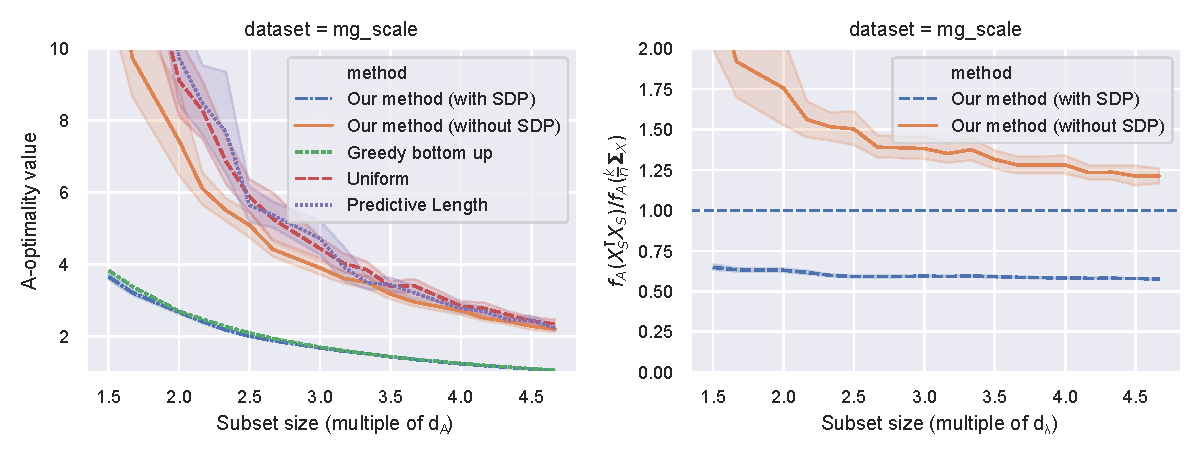
\includegraphics[width=\textwidth]{aistats/Figures/mg_combined.pdf}
     % 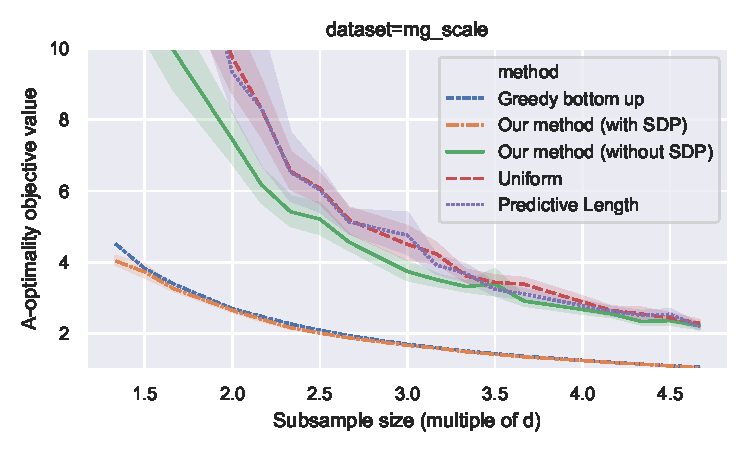
\includegraphics[width=0.51\textwidth]{bayesian_figures/objectives-mg_scale-full.pdf}\hspace{-2mm}\nobreak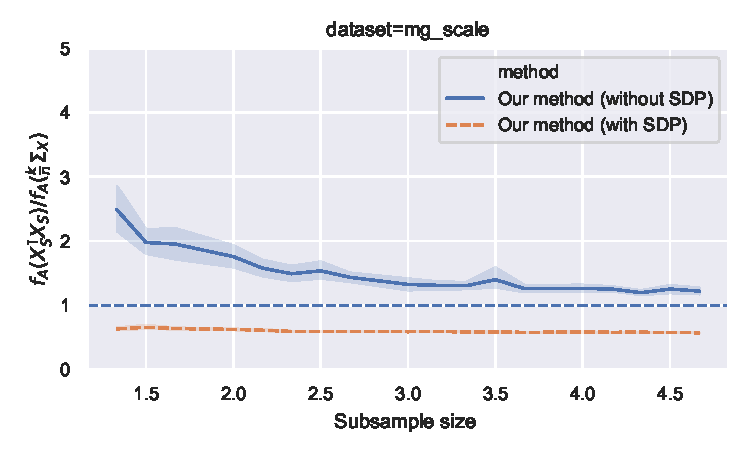
\includegraphics[width=0.51\linewidth]{bayesian_figures/ratios-mg_scale.pdf}
    % 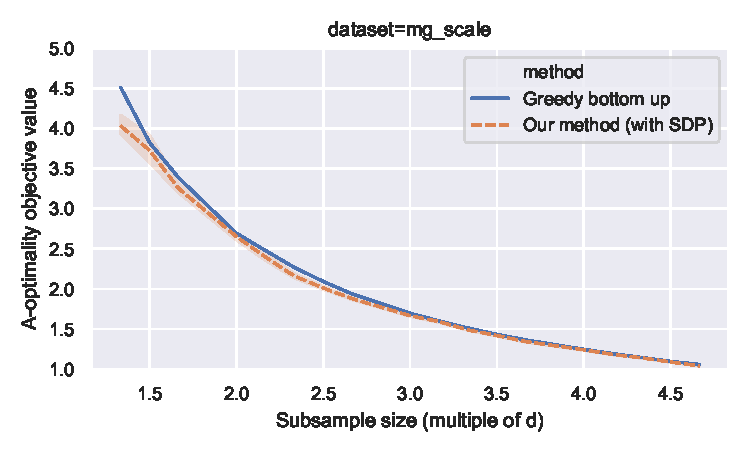
\includegraphics[width=0.49\textwidth]{bayesian_figures/objectives-mg_scale-zoom.pdf}
    \caption{(left) A-optimality value obtained by the various methods on
        the \texttt{mg\_scale} dataset \cite{libsvm} with
        prior precision $\A = 10^{-5}\, \I$,\quad (right)
A-optimality value for our method (with and without SDP) divided by
$f_{\A}(\frac kn\Sigmab_{\X})$, the baseline estimate suggested by Theorem \ref{t:q1}.}
    \label{f:experiments}
\end{figure*}


\section{Experiments}\label{s:experiments}

In this section we demonstrate that our method is capable of finding better
experimental designs $S \subset [n]$ on data matrices $\X$ occuring in on real
world data from \texttt{libsvm} datasets \citep{libsvm} (more details in
Appendix~\ref{a:experiments}).
We compare our method against the following baselines and recently proposed methods
for A-optimal design that have been shown to perform well in
practice:
\begin{description}
    \item[Our method (with SDP)] uses the efficient algorithms
        developed in proving Theorem~\ref{t:q2} to sample
        $\DPPreg{p}(\X,\A)$ constrained to subset size $k$
        with $p = w^*$, see \eqref{eq:sdp},
        obtained using a         recently developed first order convex cone solver called Splitting
        Conical Solver (SCS) \citep{o2016conic}.
        We chose SCS because it can handle the SDP constraints in
        \eqref{eq:sdp} and has provable termination guarantees, while
        also finding solutions faster \citep{o2016conic} than alternative
        off-the-shelf optimization software libraries such as SDPT3 and Sedumi.

    \item[Our method (without SDP)] samples $\DPPreg{p}(\X,\A)$ with uniform
      probabilities $p \equiv \frac{k}{n}$.
      % Compared to uniform and predictive length
      %   sampling, there is an additional DPP sampling overhead which is independent
      %   of sample size $k$ (but does depend on $d$).

          \item[Greedy bottom-up] adds an index $i \in [n]$ to the sample $S$
        maximizing the increase in A-optimality criterion
        \citep{greedy-supermodular,chamon2017approximate}.
       %  This method posesses well-understood theoretical bounds
       %  (however they
       % require additional assumptions on the matrix $\X$) and has strong
       %  empirical performance \cite{tractable-experimental-design}.

    \item[Uniform] samples every size $k$ subset $S \subseteq [n]$
        with equal probability.

    \item[Predictive length] sampling \citep{zhu2015optimal} samples
        each row $\x_i$ of $\X$ with probability $\propto\|\x_i\|$.
\end{description}

\subsection{Bayesian A-optimal design}

Consistent with prior work \citep{mariet2017elementary,chaloner1984optimal}
in optimal Bayesian experimental design,
we consider the task of A-optimal design:
given a data matrix $\X \in \R^{n \times d}$, select
$S \subset [n]$ of size $\lvert S \rvert = k$ such that
the A-optimality
criterion,
\[f_{\A}(\X_S^\top \X_S) = \tr \left((\X_S^\top \X_S + \A)^{-1}\right),\]
is small.
All our experiments set the prior precision matrix to $\A = n^{-1} \I$
and we consider sample sizes $k \in [d, 5d]$.
Each experiment is averaged over 25 trials and bootstrap 95\% confidence
intervals are shown.

Figure~\ref{f:experiments} reveals that our method (without SDP) is superior
to both uniform and predictive length sampling, producing designs which
achieve lower $A$-optimality criteria values for all sample sizes.
As Theorem~\ref{t:algorithm} shows that our method (without SDP) only differs
from uniform sampling by an additional DPP sample with controlled
expected size (see Lemma~\ref{l:size}), we may conclude
that adding even a small DPP sample can improve a uniformly sampled design.

Consistent with prior observations
\citep{chamon2017approximate,tractable-experimental-design}, the greedy bottom up
method achieves surprisingly good performance, despite the limited
theoretical guarantees it offers. However, if our method is used
in conjunction with an SDP solution, then we are able to match and
even slightly exceed the performance of the greedy bottom up
method. Furthermore, the overall run-time costs (see Appendix~\ref{a:experiments})
between the two are comparable. As the majority of the runtime of our
method (with SDP) is occupied by solving the SDP, an interesting future direction
is to investigate alternative solvers such as interior point methods as well
as terminating the solvers early once an approximate solution is reached.

Figure~\ref{f:experiments} (right) numerically evaluates the tightness of the
bound obtained in Theorem \ref{t:q1} by plotting the ratio:
\[\frac{f_{\A}(\X_S^\top \X_S)}{ f_{\A}(\frac{k}{n}\Sigmab_\X)}\]
for subsets returned by our method (with and without SDP). Note that the
line for our method with SDP on
Figure~\ref{f:experiments} (right) shows that the ratio never goes
below 0.5, and we saw similar behavior across all examined datasets
(see Appendix~\ref{a:experiments}). This evidence suggests that for
    many real datasets $\opt$ is within only a small constant factor
    away from $f_{\A}(\frac{k}{n}\Sigmab_\X)$, matching the upper bound of
    Theorem~\ref{t:q1}.
% As sample size $k \to n$, this should converge towards $1$ because $\X_S^\top
% \X_S \to \X^\top \X = \Sigma_X$.
% Across all datasets we examined, we see that this ratio is close to
% its asymptotic value of $1$. Similar to how condition
% numbers are the proper problem dependent constants in matrix inversion
% \cite{nocedal2006numerical}
% and $\tr (\frac{k}{n} \X^\top \X)^{-1}$
% is the problem-dependent constant which appear in results on non-Bayesian
% experimental design \feynman{Citation for this COLT paper?}, our results here
% suggest that $f_{\A}\left(\frac{k}{n} \X^\top \X\right)$
% is the proper problem-dependent constant for Bayesian optimal experimental
% design with a $k$ cardinality constraint.
% \feynman{Does this make sense?}


\subsection{Subsampled ridge regression}

\begin{figure}[htbp]
    \centering
    % \hspace{-0.85cm}
    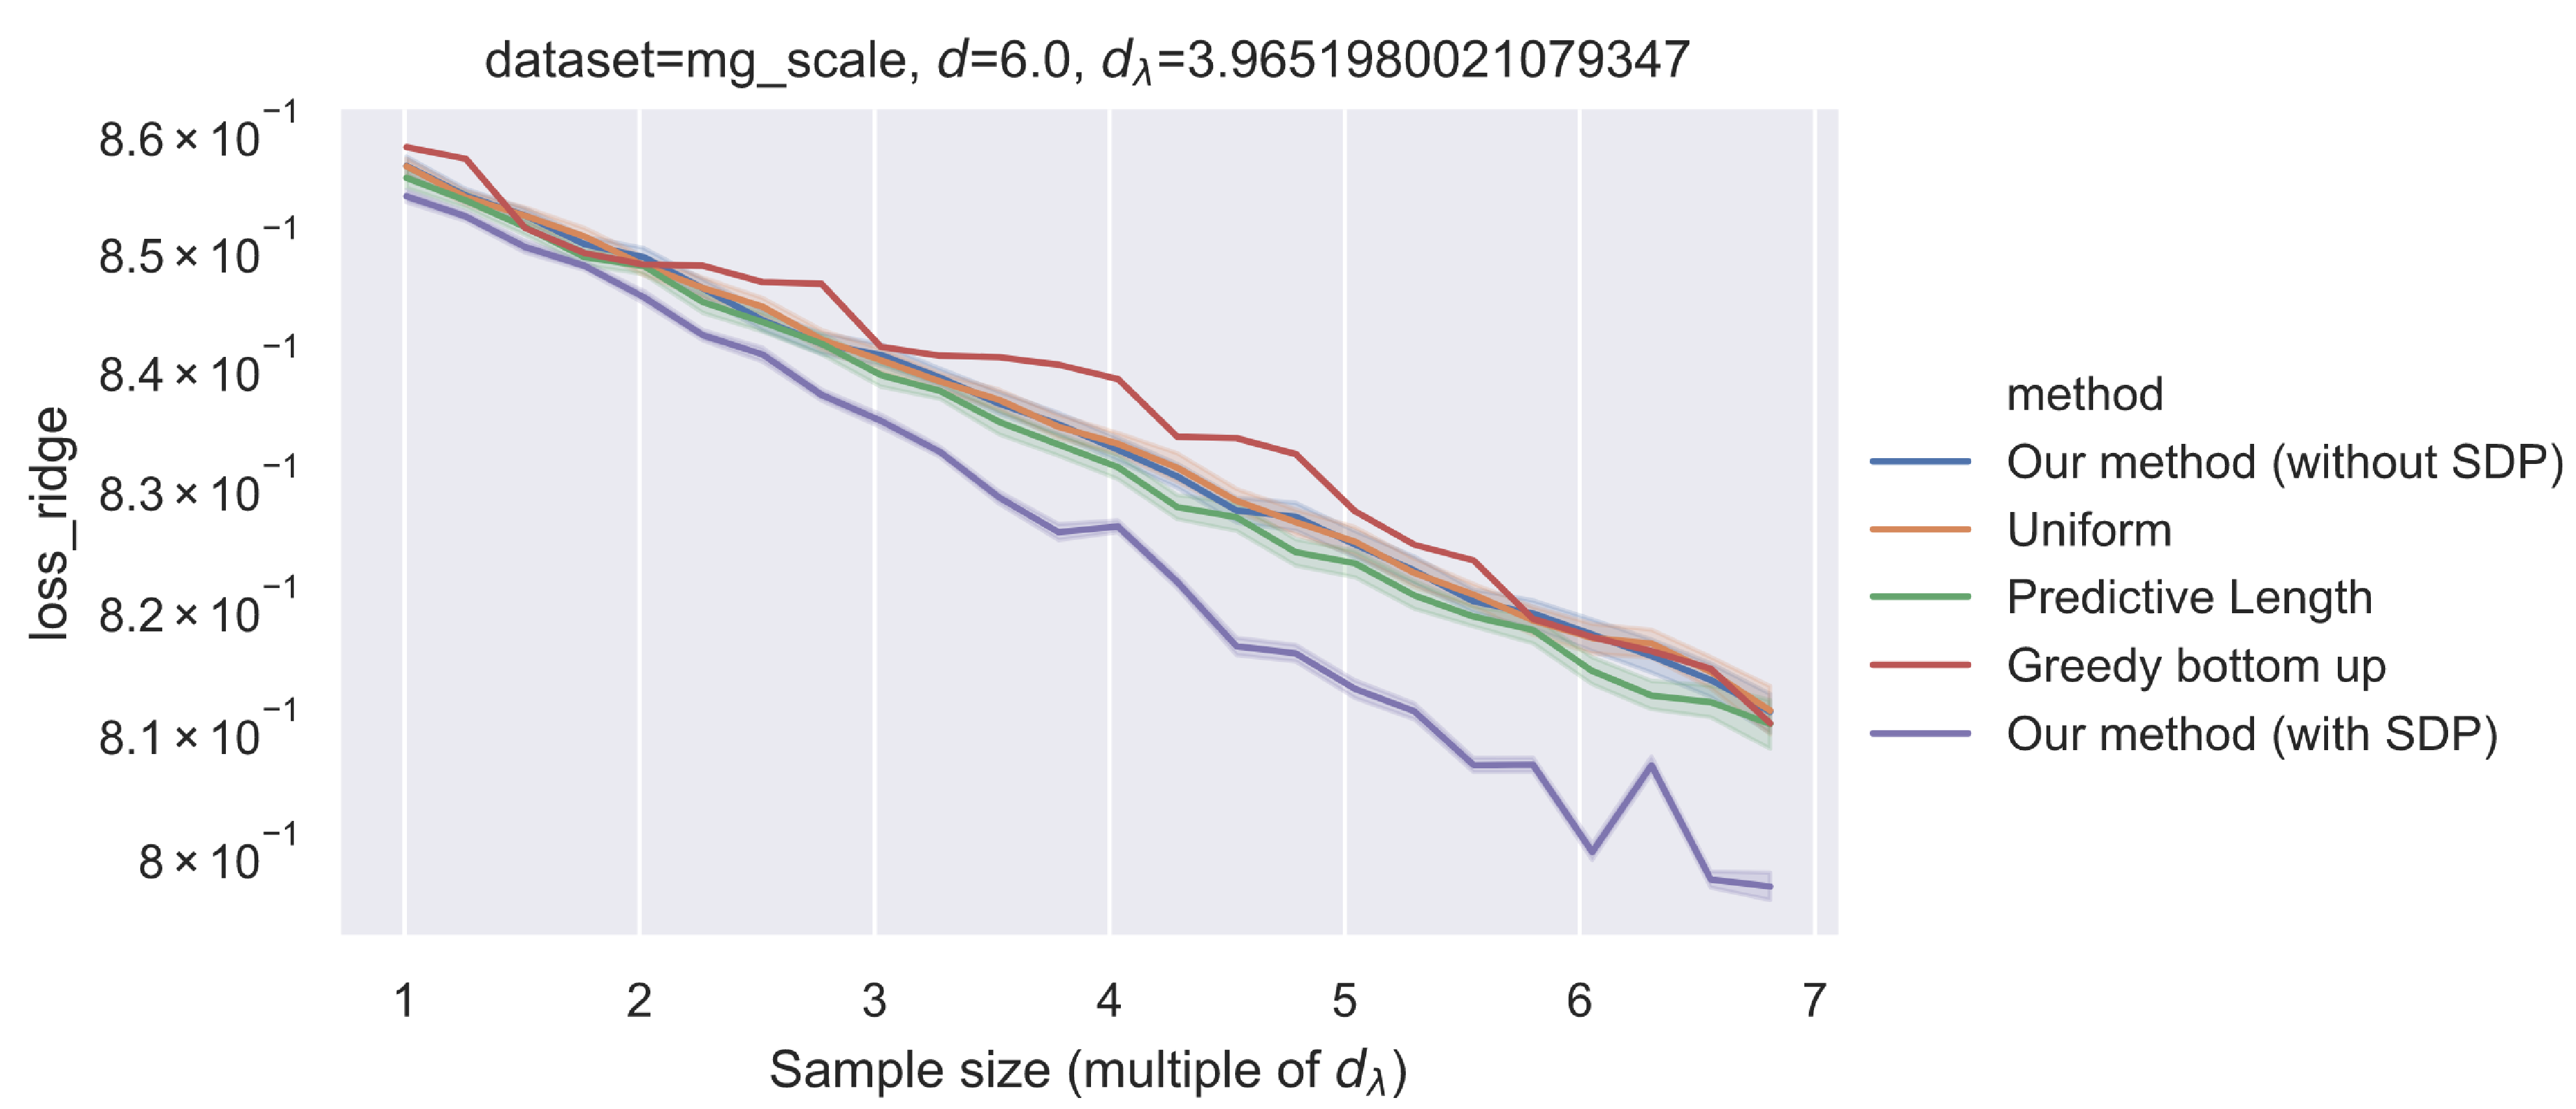
\includegraphics[width=0.8\textwidth]{bayesian_figures/mg_scale_ridge.pdf}
    \caption{Mean-squared error for subsampled ridge estimates
        on \texttt{mg\_scale}
    }
    \label{fig:low_d_eff}
\end{figure}

As experimental design is oftentimes employed as a data reduction step within a
predictive modelling pipeline, we validate the practical utility of our
algorithm by demonstrating superior performance for row subset selection in a
ridge regression task on $\texttt{mg\_scale}$.
We chose $\A = \lambda \I$ such that $\approx 95\%$ of the spectral mass was
contained in eigenvalues exceeding $\lambda$, resulting in an effective
dimension $d_\A \approx 3.97 \ll 6 = d$.  Because $d_\A$ is smaller than $d$,
the new theoretical results in this paper (Theroem~\ref{t:q1}) provide tighter
guarantees than previous bounds which depended only on $d$.

We first use the various methods to produce a design $S \subset [n]$,
form the subsampled ridge estimator $\hat{\w}_S = (\X_S^\top \X_S + \A)^{-1}
\X_S^\top \y_S$ (which is also the posterior mean of $\w$ given $\y_S$),
and plots its $\ell_2$ distance from the full unsubsampled
estimator $\hat{\w}_{[n]}$ (i.e. the posterior mean of $\w$ given $\y_{[n]}$)
in Figure~\ref{fig:low_d_eff} ($100$ trials with $95\%$ confidence intervals).
Our method outperforms all of the other methods compared, achieveing a lower
relative approximation error as the sample size increases.
